%%% LaTeX Template: Two column article
%%%
%%% Source: http://www.howtotex.com/
%%% Feel free to distribute this template, but please keep to referal to http://www.howtotex.com/ here.
%%% Date: February 2011

%%% Preamble
\documentclass[	DIV=calc,%
							paper=a4,%
							fontsize=12pt,%
							onecolumn]{scrartcl}	 					% KOMA-article class

\usepackage{lipsum}													% Package to create dummy text
\usepackage[brazil]{babel}										% English language/hyphenation
\usepackage[protrusion=true,expansion=true]{microtype}				% Better typography
\usepackage{amsmath,amsfonts,amsthm}					% Math packages
\usepackage[pdftex]{graphicx}									% Enable pdflatex
\usepackage[svgnames]{xcolor}									% Enabling colors by their 'svgnames'
\usepackage[hang, small,labelfont=bf,up,textfont=it,up]{caption}	% Custom captions under/above floats
\usepackage{epstopdf}												% Converts .eps to .pdf
\usepackage{subfig}													% Subfigures
\usepackage{booktabs}												% Nicer tables
\usepackage{fix-cm}													% Custom fontsizes
\usepackage[utf8]{inputenc}
\usepackage[top=2.5cm, bottom=2.5cm, left=1cm, right=1cm]{geometry}
\usepackage[ddmmyyyy]{datetime}
\addto\captionsenglish{%
	\renewcommand\tablename{Tabela}
	\renewcommand\figurename{Figura}
} 
 

 
%%% Custom sectioning (sectsty package)
\usepackage{sectsty}													% Custom sectioning (see below)
\allsectionsfont{%															% Change font of al section commands
	\usefont{OT1}{phv}{b}{n}%										% bch-b-n: CharterBT-Bold font
	}

\sectionfont{%																% Change font of \section command
	\usefont{OT1}{phv}{b}{n}%										% bch-b-n: CharterBT-Bold font
	}



%%% Headers and footers
\usepackage{fancyhdr}												% Needed to define custom headers/footers
	\pagestyle{fancy}														% Enabling the custom headers/footers
\usepackage{lastpage}	

% Header (empty)
\lhead{}
\chead{}
\rhead{}
% Footer (you may change this to your own needs)

%% ====================================
%% ====================================
%% mude o rodape  do projeto
%% ====================================
%% ====================================

\lfoot{\footnotesize \texttt{Cabeamento Estruturado} \textbullet ~Projeto - D.H.U Contabilidade e Assessoria LTDA}


\cfoot{}
\rfoot{\footnotesize página \thepage\ de \pageref{LastPage}}	% "Page 1 of 2"
\renewcommand{\headrulewidth}{0.0pt}
\renewcommand{\footrulewidth}{0.4pt}



%%% Creating an initial of the very first character of the content
\usepackage{lettrine}
\newcommand{\initial}[1]{%
     \lettrine[lines=3,lhang=0.3,nindent=0em]{
     				\color{DarkGoldenrod}
     				{\textsf{#1}}}{}}



%%% Title, author and date metadata
\usepackage{titling}															% For custom titles

\newcommand{\HorRule}{\color{DarkGoldenrod}%			% Creating a horizontal rule
									  	\rule{\linewidth}{1pt}%
										}

\pretitle{\vspace{-30pt} \begin{flushleft} \HorRule 
				\fontsize{50}{50} \usefont{OT1}{phv}{b}{n} \color{DarkRed} \selectfont 
				}

%% ====================================
%% ====================================
%% mude o titulo  do projeto
%% ====================================
%% ====================================

\title{Projeto de cabeamento estruturado da empresa D.H.U Contabilidade e Assessoria LTDA}					% Title of your article goes here

%% ====================================



\posttitle{\par\end{flushleft}\vskip 0.5em}

\preauthor{\begin{flushleft}
					\large \lineskip 0.5em \usefont{OT1}{phv}{b}{sl} \color{DarkRed}}
\author{Thiago Mitsuo Yamada}  	% Author name goes here


\postauthor{\footnotesize \usefont{OT1}{phv}{m}{sl} \color{Black} 
					\\Universidade Tecnológica Federal do Paraná - Câmpus Cornélio Procópio 								% Institution of author
					\par\end{flushleft}\HorRule}

\date{}																				% No date




%%% Begin document
\begin{document}
\maketitle
\thispagestyle{fancy} 	
\thispagestyle{empty}		% Enabling the custom headers/footers for the first page 
% The first character should be within \initial{}




%% ====================================
%% ====================================
%% mude o resumo  do projeto
%% ====================================
%% ====================================
\initial{O}\textbf{objetivo do projeto será a criação de uma estrutura completamente nova de cabeamento estruturado para a empresa D.H.U Contabilidade e Assessoria LTDA. Essa nova estrutura será composta por diversos computadores, além de servidores de aplicação e backup. Todos os computadores serão interligados a um domínio, controlados pelo Active Directory, oferecido pelo sistema operacional Windows Server. Os usuários serão vinculados a este controlador de domínio e possuirão acesso a um terminal service. O projeto abrange todo o levantamento de planta física, elaboração da planta logica, levantamento dos equipamentos de informática e o orçamento da implantação.  }

%% ====================================
\begin{figure}
	\centering
	\includegraphics{utfpr}
\end{figure}

\vspace{1cm}
\centerline{\textit{\textbf{\today}}}

\clearpage
    \renewcommand*\listfigurename{Lista de figuras}
\listoffigures

\renewcommand*\listtablename{Lista de tabelas}
\listoftables




\clearpage
\renewcommand{\contentsname}{Sumário}
\tableofcontents
\clearpage

%% ====================================
%% ====================================
%% Inicio do texto
%% ====================================
%% ====================================
\section{Introdução}
A empresa atualmente está transitando para uma nova instalação, com estrutura predial mais moderna, atendendo aos requisitos para o projeto de cabeamento estruturado. Na estrutura atual, a empresa não possui nenhum sistema de cabeamento estruturado, e com o aumento no quadro de funcionários, a rede tornou-se instável, com muitos problemas de conexão e baixa velocidade.

O quadro de funcionários conta com 8 funcionários, divididos nas áreas de pessoa física, pessoa jurídica, gerência e arquivo morto. Os equipamentos de TI são constituídos em 9 computadores, 1 roteador, 1 switch e 2 impressoras. 

O escopo do projeto constitui a instalação física de toda a parte do cabeamento e equipamentos de TI, além de sua configuração, documentação completa, testes funcionais e a realização da certificação.

A expansão prevista da empresa não será maior que 30 computadores.

\subsection{Benefícios}
Os benefícios com a introdução de uma estrutura de cabeamento estruturado resultará em maior estabilidade para a rede, além da facilidade na manutenção, segurança para os funcionários e clientes, a possibilidade da execução de aplicativos de forma remota e o aumento do desempenho das atividades da empresa. 

\subsection{Organizações Envolvidas}
As organizações envolvidas no projeto de cabeamento estruturado são apresentadas na tabela \ref{tab7} abaixo:

\begin{table}[h!]
	\centering
	\caption{Organizacoes envolvidas.}
	\label{tab7} %com este label vc faz referencia no texto
	
\begin{tabular}{|c|c|}
\hline
Organizacao Envolvida         & Area Responsavel                                                                                                   \\ \hline
Equipe 1                      & Desenvolvimento do projeto e comunicacao com o cliente                                                             \\ \hline
Equipe 2                      & Passagem de cabos e crimpagem de conectores                                                                        \\ \hline
Equipe 3                      & Montagem de racks, servidores, switches e patch panels                                                             \\ \hline
Equipe 4                      & \begin{tabular}[c]{@{}c@{}}Montagem de Eletrocalhas, tomadas de rede e \\ identificacao do cabeamento\end{tabular} \\ \hline
Equipe 5                      & Certificacao da rede                                                                                               \\ \hline
Equipe 6 - Empresa Contratada & Configuracao de servidores, micros e impressoras                                                                   \\ \hline
Equipe 7 - Construtora        & Responsavel pela construcao do predio comercial                                                                    \\ \hline
\end{tabular}
\end{table}





































\section{Estado atual}

Atualmente o estado da rede é composta por uma pequena estrutura, constituindo de 1 roteador, 9 computadores, 1 switch, 2 impressoras e os cabos cat5 para a conexão entre os equipamentos de TI.

As principais reclamações dos funcionários baseiam-se nos problemas quanto a estabilidade da conexão. Muitos dos aplicativos utilizados sofrem com a queda da conexão e dessa forma gerando transtornos para a finalização dos serviços. Além disso a manutenção é dificultada por não possuir uma estrutura organizada.

\section{Requisitos}

Os requisitos do projeto são:

1- Possibilidade de expansão da rede para compra de novos equipamentos;

2- Serviço de controle de usuários;

3- Bloqueio de acesso a sites com conteúdo inapropriado;

4- Serviço de segurança das informações trafegadas na rede;

5- Serviço de cópia de segurança dos dados utilizados;

6- Serviço de acesso remoto para uso de aplicativos.

\section{Usuários e Aplicativos}
A situação atual da empresa consiste no quadro de 8 funcionários, todos com computadores individuais. A estimativa com à mudança de prédio, é contratar até 4 funcionários para as novas necessidades. Além disso, para uma demanda futura, a empresa prevê à contratação de estagiários para compor o quadro de funcionários. Considerando a evolução prevista, o projeto prevê a instalação de no máximo 60 pontos de rede, além da compra de 3 servidores, 4 switches, 4 patch panels , 4 computadores, 2 roteadores wifi e 1 impressora, para a atual mudança de prédio.

\subsection{Usuários}
Os perfis de usuário são compostos por 8 funcionários, divididos em dois para o escritório de gerência, um para o arquivo morto, dois para o escritório de pessoa física e mais dois no de pessoa jurídica.

\subsection{Aplicativos}
Os aplicativos utilizados pelo escritório com uso intenso são:

- Pacote Office da Microsoft, principalmente o Excel e o pacote LibreOffice, utilizando o aplicativo Calc.

- Aplicativos destinados a declaração para Receita Federal, Receita Estadual, Municipais e para declarações trabalhistas.

Os demais aplicativos utilizados pelo escritório são de uso tradicional, como navegadores de internet.


\section{Estrutura predial existente}
A nova estrutura predial é apresentado na figura \ref{fisica1} abaixo. O prédio apresenta uma área total de 261.9 metros quadrados, possuindo as seguintes divisões na estrutura: sala de telecomunicações, com 10.5 metros quadrados; sala de equipamentos, com 18.6 metros quadrados; escritório de gerência, com 38.25 metros quadrados; escritório de pessoa física, com 51 metros quadrados; escritório de pessoa jurídica, com 59.5 metros quadrados; arquivo morto, com 34 metros quadrados e a recepção, com 24.25 metros quadrados. Todas as salas serão interligadas através do corredor, iniciando a partir da recepção, possuindo 25.8 metros quadrados de área.

\begin{figure}[h]
	\centering
	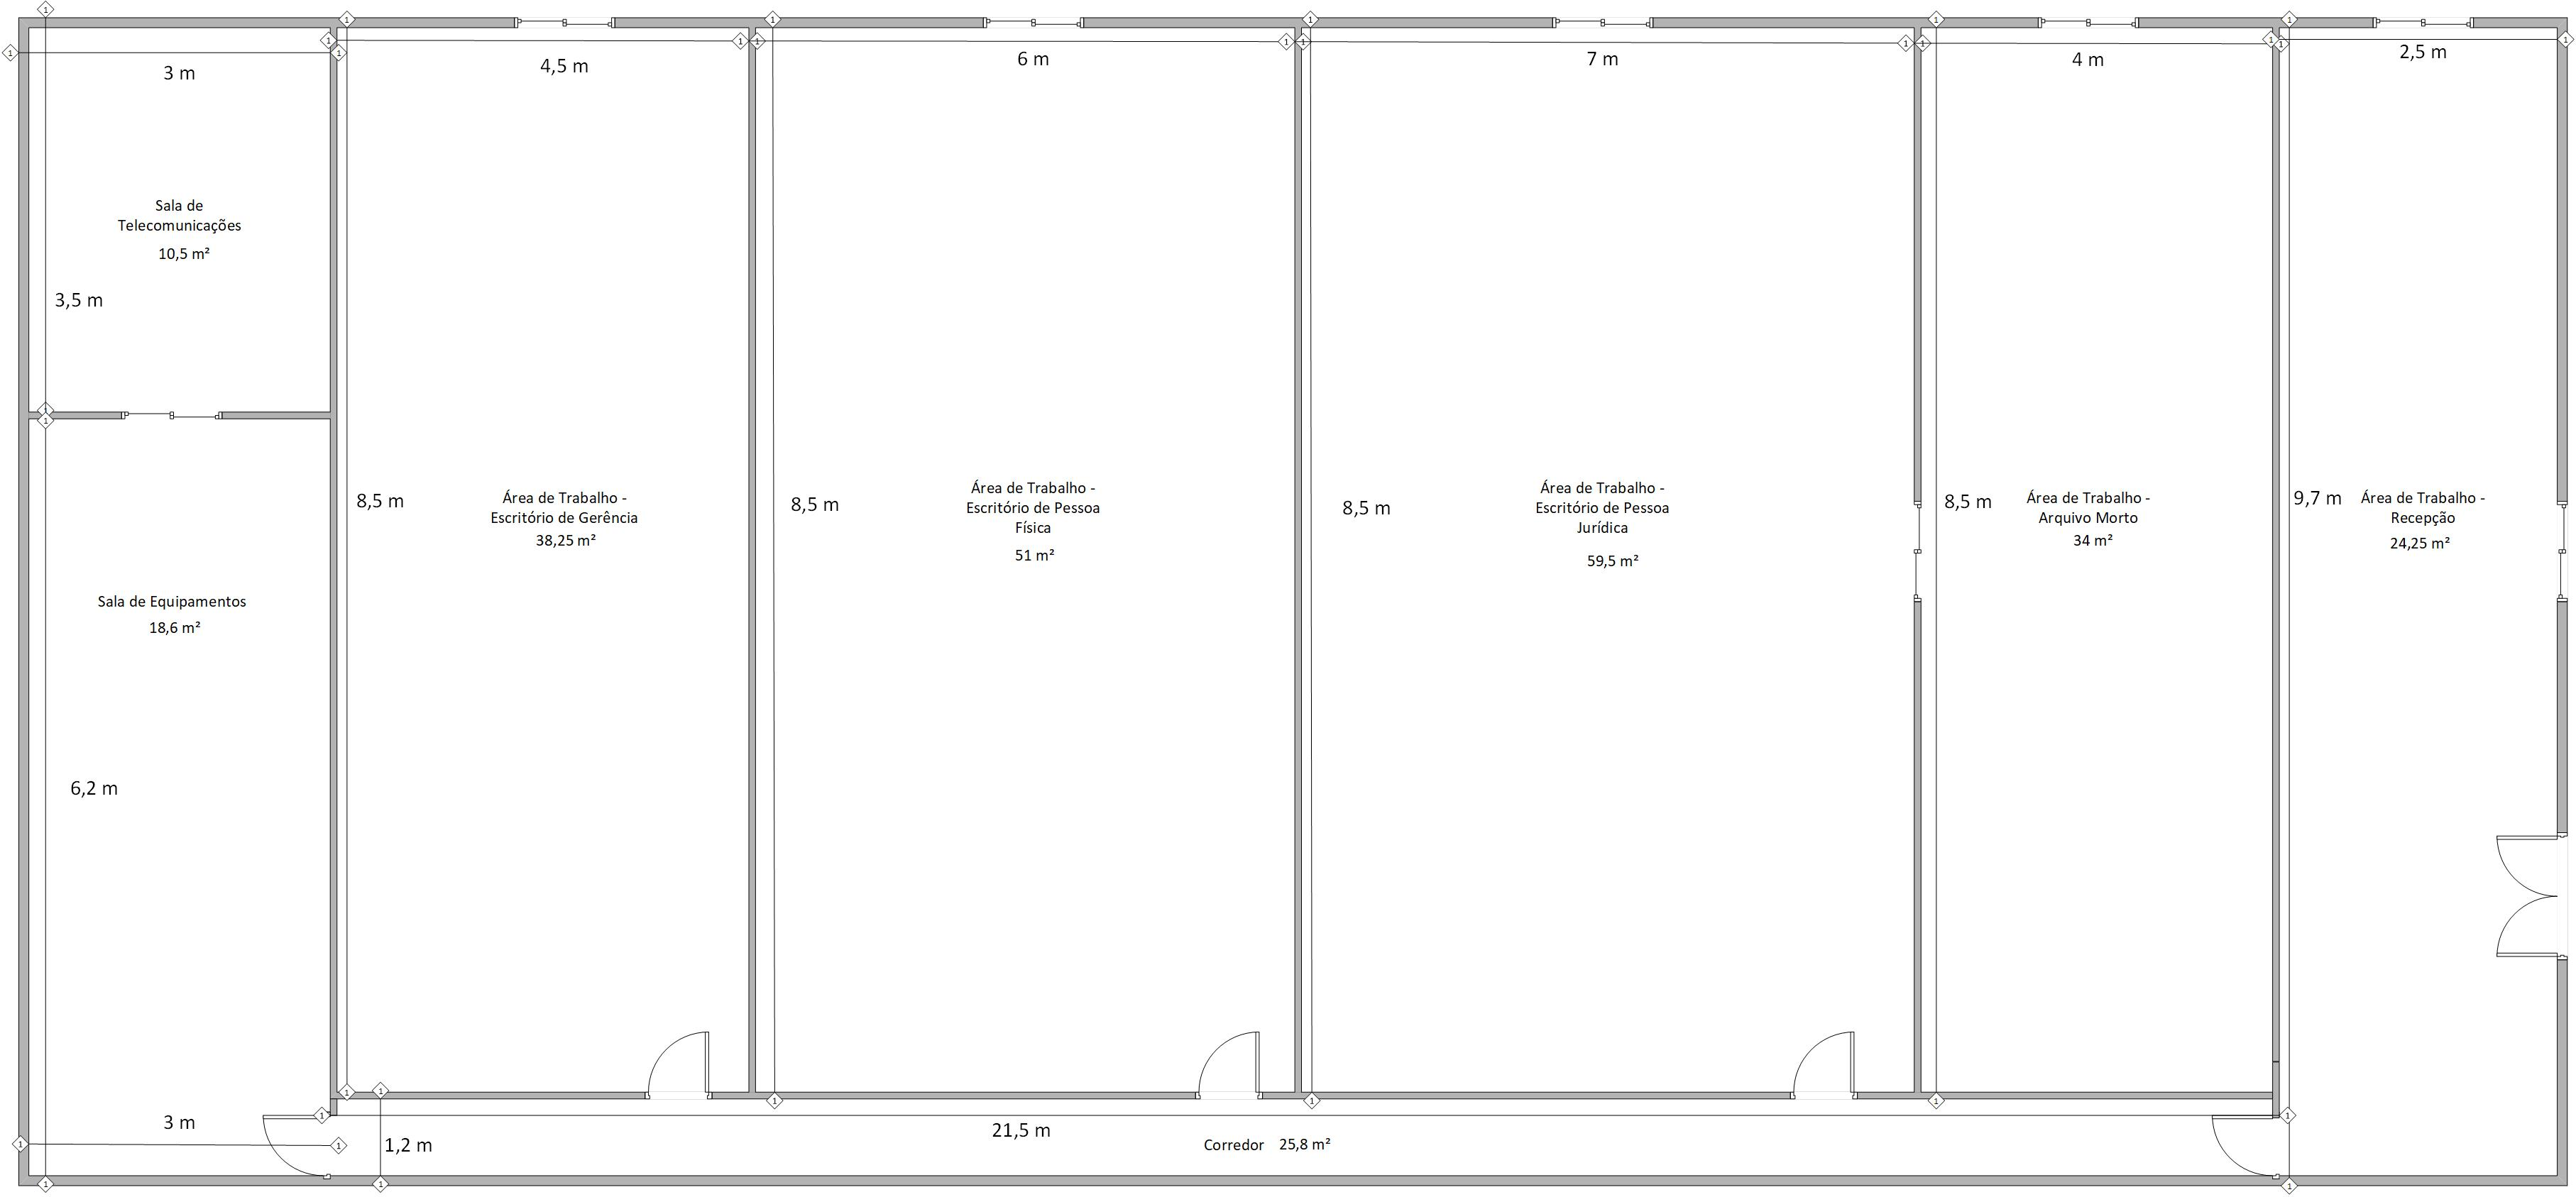
\includegraphics[scale=0.23]{fisica1}
	\caption{Planta Física do prédio.}
	\label{fisica1}
\end{figure} 

O projeto abrange uma estrutura que disponibilizará eletrodutos para o alojamento dos cabos de rede através das paredes e os compartimentos para os pontos de rede. Além disso, a estrutura predial utiliza teto falso entre a laje, facilitando o uso de eletrocalhas para a distribuição do cabeamento de rede.

As distancias entre os pontos de rede podem variar entre 1 a 3 metros de distância.

\section{Planta Lógica - Elementos estruturados}

\subsection{Estado atual}
O estado atual da rede encontra-se composta por 9 computadores, 1 switch de 100 megabits, 1 roteador e o cabeamento utilizando cabos cat5. Os equipamentos como switch e roteador estão alocados em um mini rack fixado na parede do escritório. Como não foi utilizado calhas ou eletrodutos, os cabos foram distribuídos de forma aleatória de acordo com a posição de cada computador, percorrendo desde eletrodutos compartilhados com fios de energia elétrica ou espalhados pelo piso do escritório.

Com a mudança de prédio, apenas os equipamentos como computadores e as impressoras serão aproveitados no novo projeto de cabeamento estruturado, os demais itens, como os cabos, serão descartados, pela necessidade de utilizar equipamentos mais modernos.

\subsection{Topologia}
A sala de TI, no qual é divida em sala de telecomunicações e em sala de equipamentos, localizam-se todos os dispositivos como modem, switches, patch panels, servidores e os racks. A recepção de internet, ilustrado no diagrama da figura \ref{diagrama1} será realizada pelo modem e em seguida para um servidor, no qual contém os serviços de proxy, dhcp, dns e active directory. Logo após, a próxima conexão será com o switch 1 ou central, este por usa vez será responsável pela conexão aos servidores de aplicação e backup, além dos switches posteriores, compondo uma topologia de rede em formato estrela. Os demais switches realizarão as conexões dos computadores situados em cada sala do prédio:
\begin{itemize}
	\item Switch 2: é encarregado da conexão dos computadores e impressora do escritório de gerência;
	\item Switch 3: é encarregado da conexão dos computadores, impressora e roteador sem fio do escritório de pessoa física;
	\item Switch 4: é encarregado da conexão dos computadores, impressora, roteador sem fio do escritório de pessoa jurídica, além do mais, da sala de arquivo morto e a recepção.
\end{itemize}

\begin{figure}[h]
	\centering
	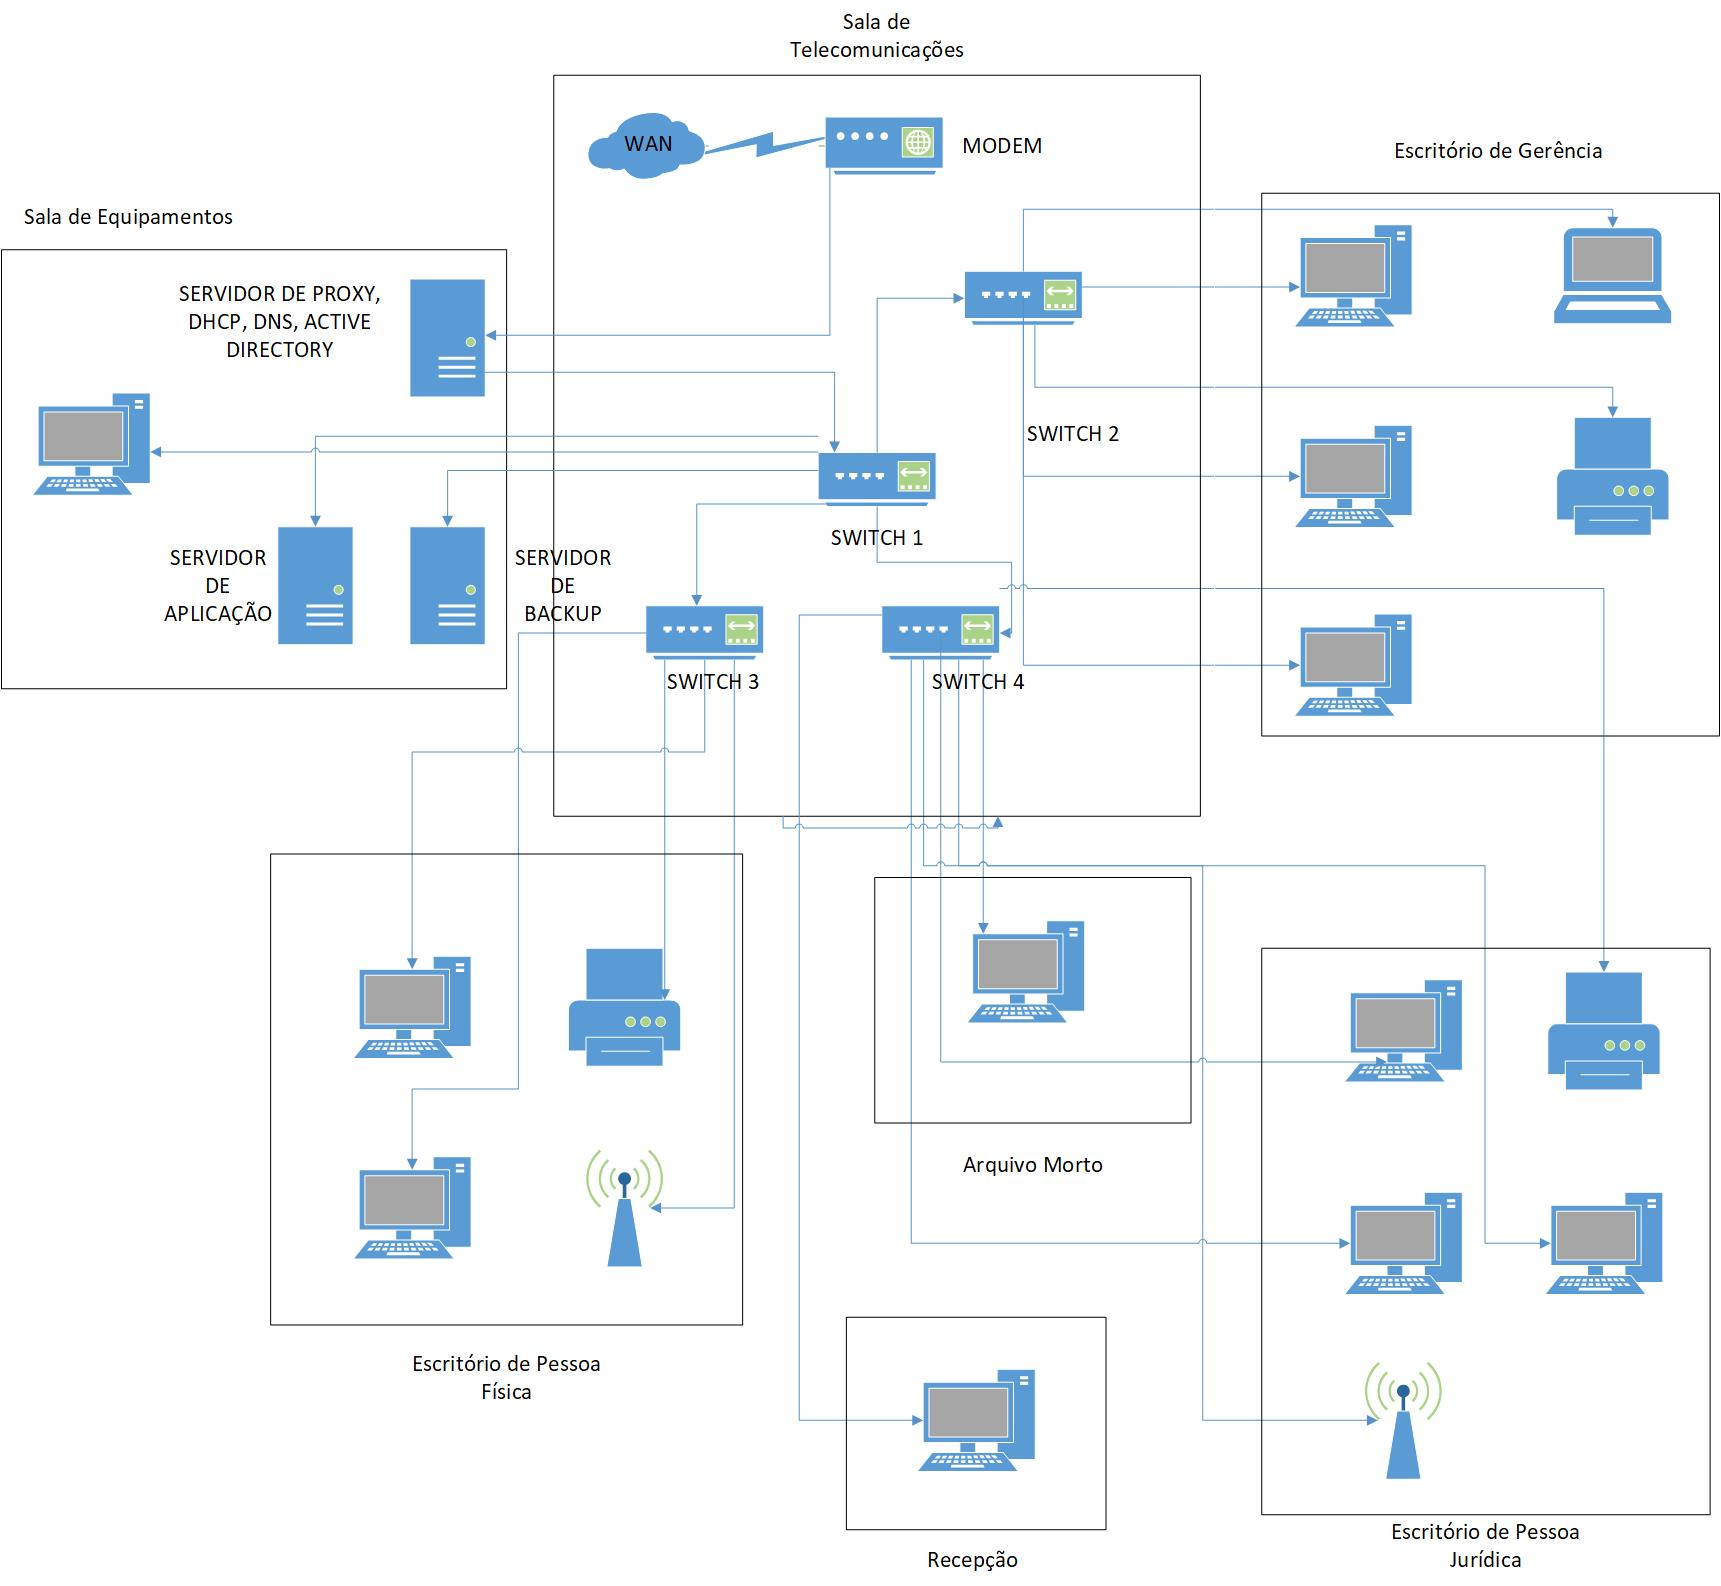
\includegraphics[scale=0.45]{diagrama1}
	\caption{Diagrama de rede.}
	\label{diagrama1}
\end{figure}

A figura \ref{desenho1} a seguir demonstra à distribuição física da rede pela estrutura do prédio. A conexão entre a rede externa e a interna é realizada por meio da entrada da edificação(facilidades de entrada), utilizando um armário de telecomunicações para abrigar os cabos da concessionária de internet, localizados na  sala de telecomunicações.

O cabeamento será todo realizado em cabos UTP categoria 6. Os switches serão todos conectados por patch cords aos patch panels, implementados em um rack. Para à conexão com as áreas de trabalhos da empresa, o projeto prevê à aplicação do sistema de cabeamento horizontal, este por sua vez, responsável pela ligação entre o patch panel e o ponto de telecomunicação específico, que no total somam 57 tomadas de rede, de acordo com o projeto estrutural do prédio.

\begin{figure}[h]
	\centering
	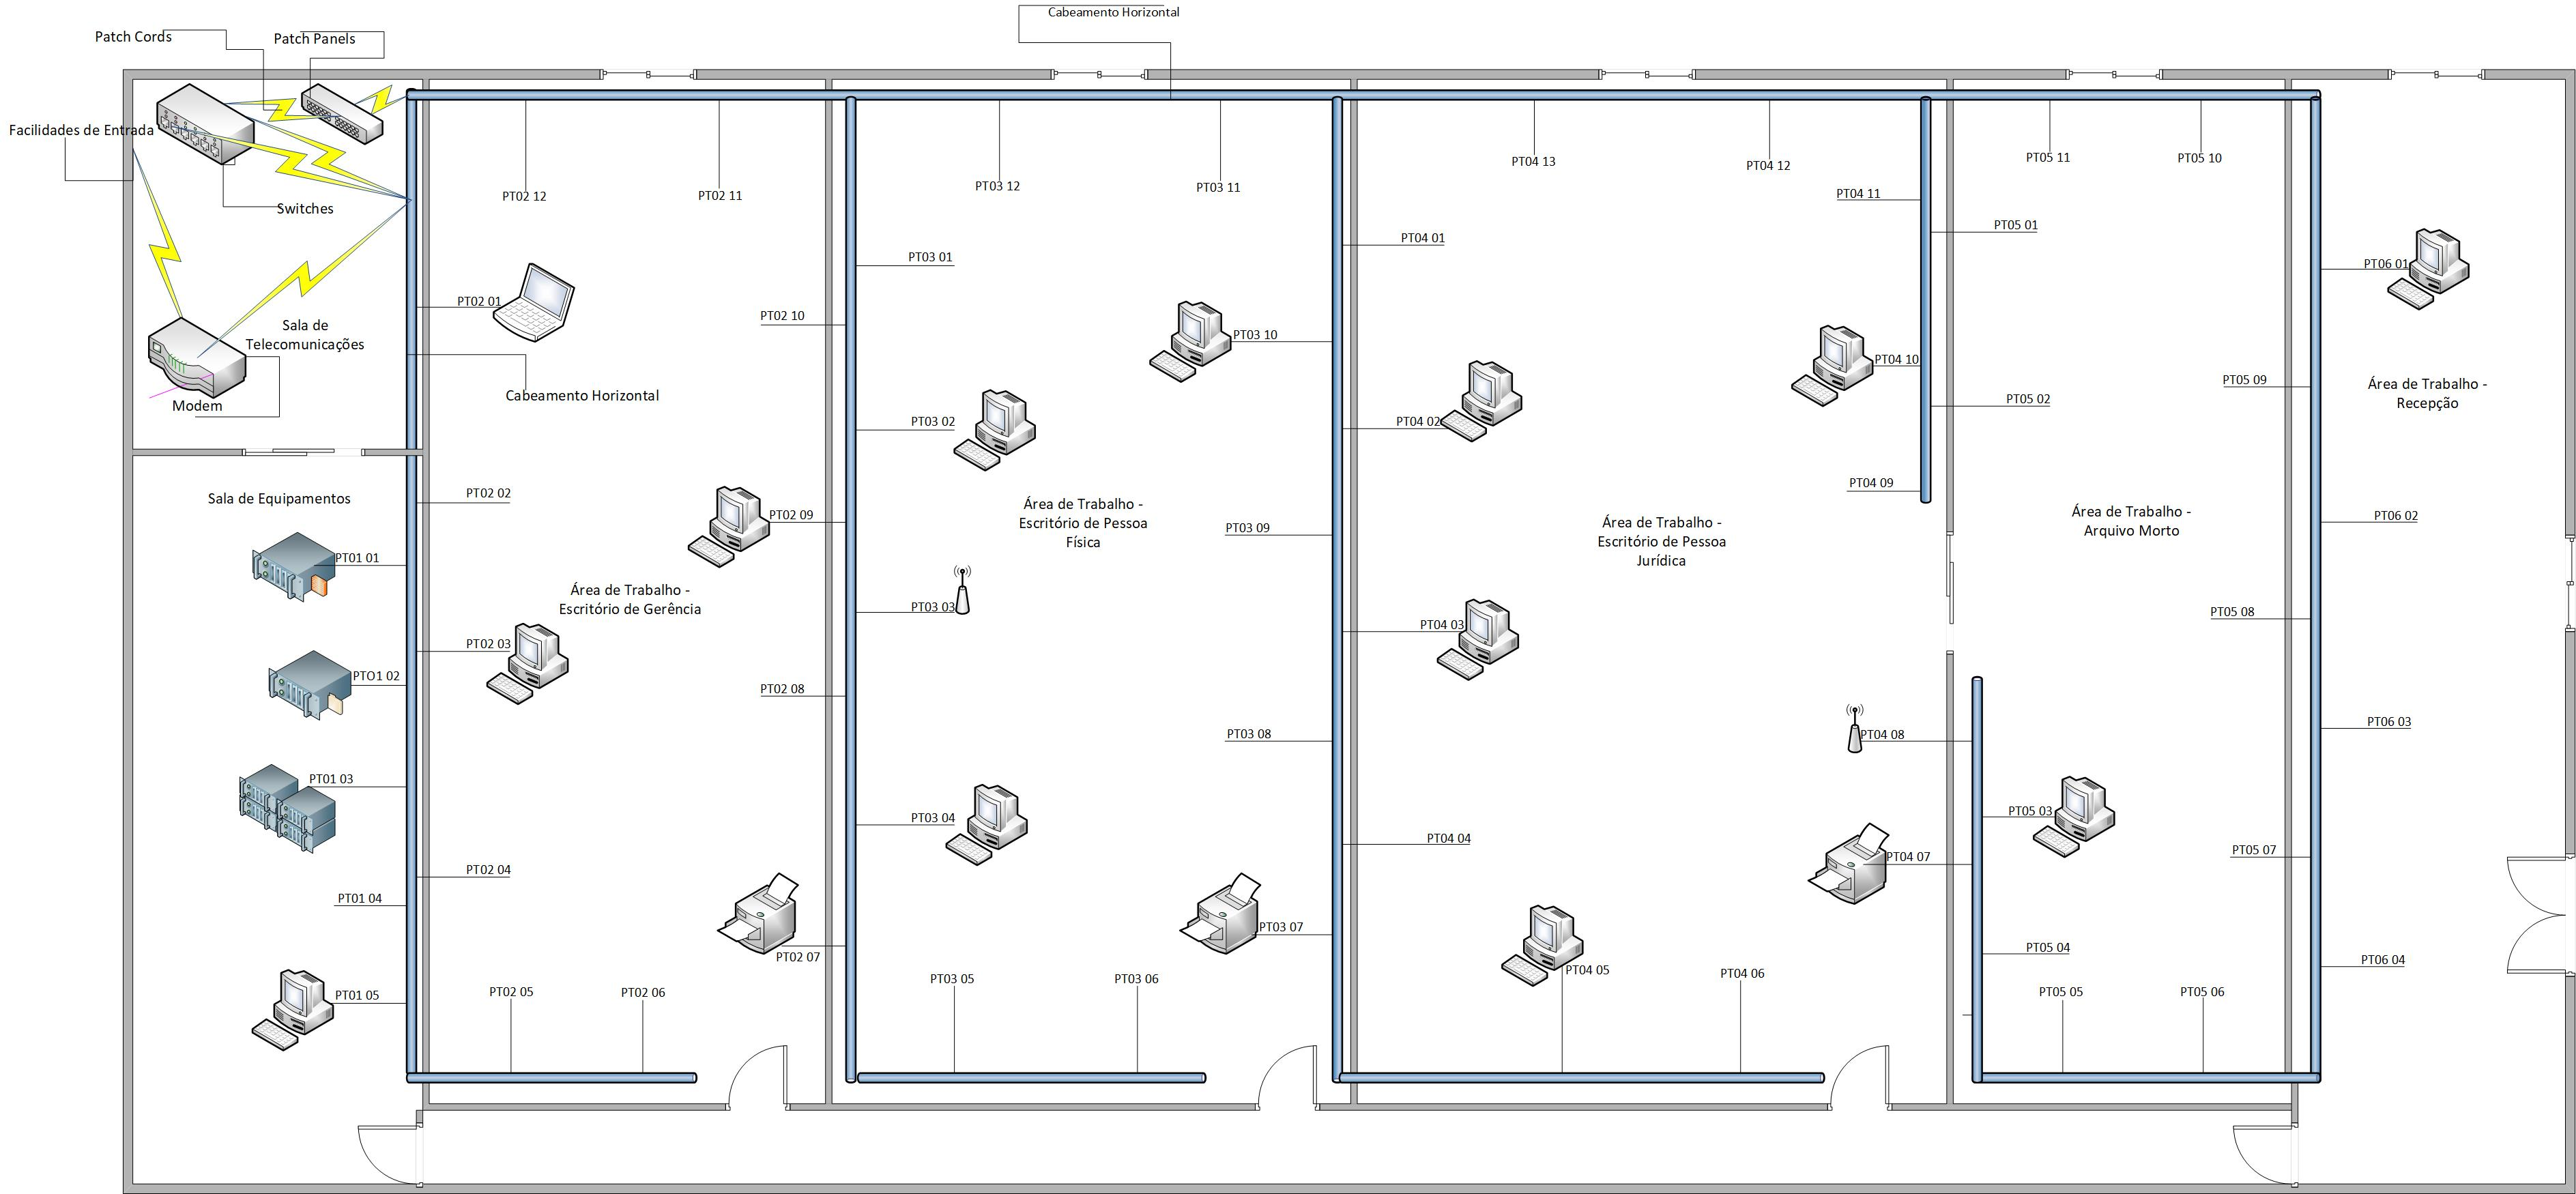
\includegraphics[scale=0.22]{desenho1}
	\caption{Diagrama da distribuição física de rede.}
	\label{desenho1}
\end{figure}

\newpage
A sala de telecomunicações abrigará um rack para alojar os switches, os patch panels e o modem de internet na seguinte configuração da figura \ref{rack2}.

\begin{figure}[h]
	\centering
	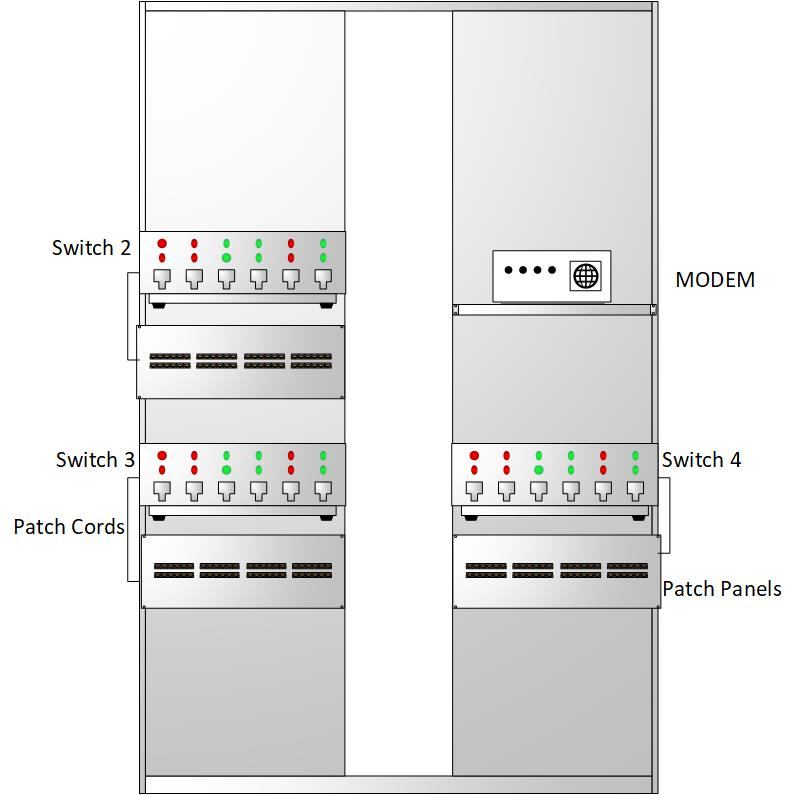
\includegraphics[scale=0.5]{rack2}
	\caption{Rack de telecomunicações.}
	\label{rack2}
\end{figure}

\newpage
A sala de equipamentos abrigará um rack para alojar o servidor de proxy, juntamente com os serviços de dhcp, dns e active directory. Bem como, os servidores de aplicação e backup, apresentados na configuração da figura  \ref{rack1}.


\begin{figure}[h]
	\centering
	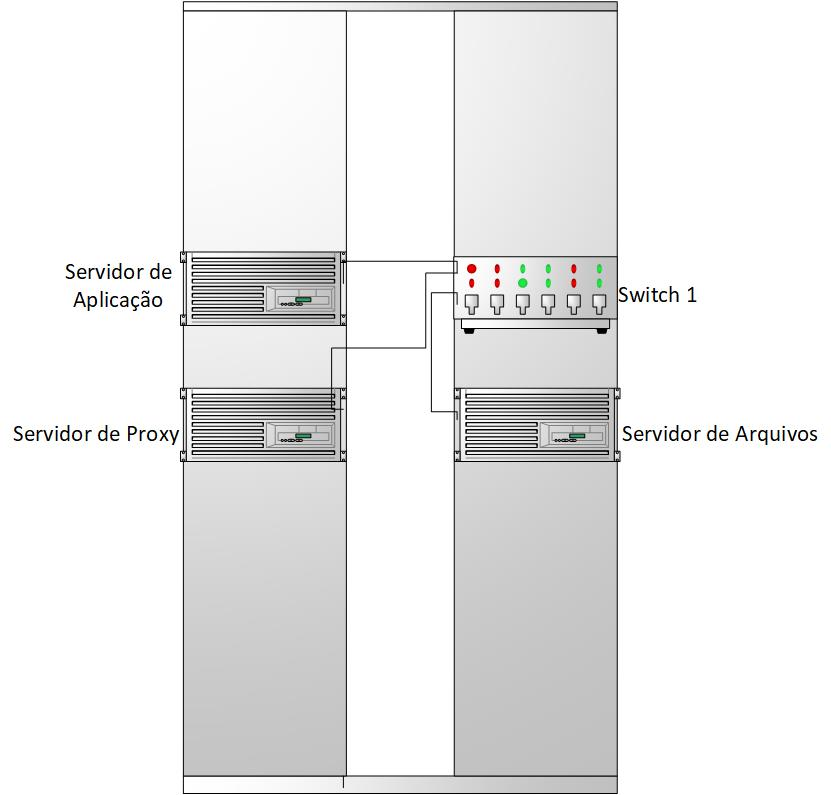
\includegraphics[scale=0.5]{rack1}
	\caption{Rack de equipamentos.}
	\label{rack1}
\end{figure}

\subsection{Encaminhamento}
O encaminhamento dos cabos será por eletrocalhas e eletrodutos, a eletrocalha fará à distribuição dos cabos pelas salas do prédio, iniciando-se desde a sala de telecomunicações, deslocando por aberturas entre as paredes dos cômodos, percorrendo através de um teto falso até a sala de recepção. 

A eletrocalha será instalada próxima a parede que contém as janelas, os eletrodutos verticais, instalados dentro das paredes, serão responsáveis pela conexão até o pequeno quadro de distribuição embutido na parede e este por sua vez será conectado aos eletrodutos horizontais, percorrendo os cabos para seus respectivos pontos de telecomunicações na sala.

\subsection{Memorial descritivo}

A tabela \ref{tab3} abaixo relaciona todos os equipamentos necessários para a nova rede, a marca, o modelo e a quantidade de ambos.

\begin{table}[h!]
	\centering
	\caption{Equipamentos Passivos de Rede}
	\label{tab3} %com este label vc faz referencia no texto
\begin{tabular}{|c|c|c|c|}
	\hline
\multicolumn{4}{|c|}{Equipamentos Passivos de Rede}                                                                                                                              \\ \hline
\multicolumn{1}{|c|}{Equipamento}                 & \multicolumn{1}{c|}{Marca}             & \multicolumn{1}{c|}{Modelo}                     & \multicolumn{1}{c|}{Quantidade} \\ \hline
\multicolumn{1}{|c|}{Cabo UTP CAT6}               & \multicolumn{1}{c|}{Furukawa}          & \multicolumn{1}{c|}{Caixa 305M}                 & \multicolumn{1}{c|}{6}          \\ \hline
\multicolumn{1}{|c|}{Patch Cords CAT6}            & \multicolumn{1}{c|}{Furukawa}          & \multicolumn{1}{c|}{Cabo 1M}                    & \multicolumn{1}{c|}{80}         \\ \hline
\multicolumn{1}{|c|}{Conector RJ-45}              & \multicolumn{1}{c|}{Furukawa}          & \multicolumn{1}{c|}{Macho CAT6 Pacote 50 Pecas} & \multicolumn{1}{c|}{3}          \\ \hline
\multicolumn{1}{|c|}{Modulo Tomada para Rede}     & \multicolumn{1}{c|}{Fame}              & \multicolumn{1}{c|}{RJ-45 CAT6 1 peca 8 vias}   & \multicolumn{1}{c|}{60}         \\ \hline
\multicolumn{1}{|c|}{Eletrocalhas}                & \multicolumn{1}{c|}{InfraEletrocalhas} & \multicolumn{1}{c|}{150x100mm - Perfuradas  3M} & \multicolumn{1}{c|}{9}          \\ \hline
\multicolumn{1}{|c|}{Eletrocalhas Curva Vertical} & \multicolumn{1}{c|}{InfraEletrocalhas} & \multicolumn{1}{c|}{Ext. 90 - 150x100mm}        & \multicolumn{1}{c|}{1}          \\ \hline
\multicolumn{1}{|c|}{Suporte Omega}               & \multicolumn{1}{c|}{InfraEletrocalhas} & \multicolumn{1}{c|}{150x100mm}                  & \multicolumn{1}{c|}{18}         \\ \hline
\multicolumn{1}{|c|}{Patch Panels}                & \multicolumn{1}{c|}{Furukawa}          & \multicolumn{1}{c|}{CAT6 24 posicoes GIGALAN}   & \multicolumn{1}{c|}{3}          \\ \hline
\multicolumn{1}{|c|}{Rack Aberto 24U}             & \multicolumn{1}{c|}{Nacional Racks}    & \multicolumn{1}{c|}{19 " - 1,27M x 0,67M}        & \multicolumn{1}{c|}{1}          \\ \hline
\multicolumn{1}{|c|}{Rack Coluna Padrao 24U}      & \multicolumn{1}{c|}{Nacional Racks}    & \multicolumn{1}{c|}{19  - 1,27M x 0,60M}          & \multicolumn{1}{c|}{1}          \\ \hline
\end{tabular}
\end{table}















 
\newpage

\subsection{Identificação dos cabos}
Para criar a identificação dos cabos de rede, foi utilizado a seguinte nomenclatura, demonstrada na figura \ref{identificacaorede}.

\begin{figure}[h]
	\centering
	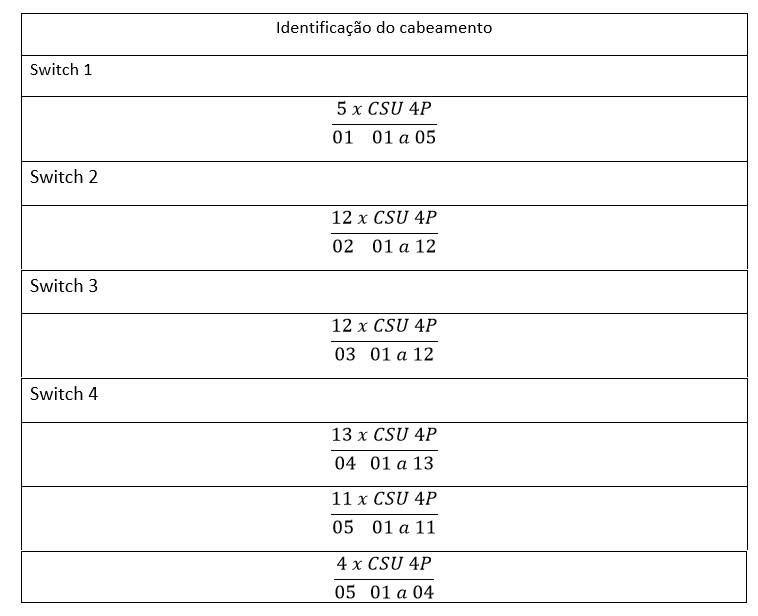
\includegraphics[scale=0.7]{identificacaorede}
	\caption{Nomenclatura da identificação dos cabos.}
	\label{identificacaorede}
\end{figure}

No switch 1, a linha "5 x CSU 4P" significa que a quantidade de cabos é 5, o cabo é secundário do tipo UTP e conta com 4 pares no fio. A linha "01 01 a 05" exibe qual área do prédio será instalado o cabeamento, no caso 01 e quais pontos de telecomunicações serão atendidos, no qual serão de 01 a 05. As demais nomenclaturas seguem a mesma lógica para a identificação do cabeamento por cada sala do prédio.

Além de identificação dos cabos por área do prédio, a nomenclatura de cada cabo em seu respectivo ponto de telecomunicações é dada pelas tabelas \ref{tab5} e \ref{tab6} abaixo.

\newpage
\begin{table}[h!]
	\centering
	\caption{Identificação de cada cabo de rede.}
	\label{tab5} %com este label vc faz referencia no texto
\begin{tabular}{|l|l|l|l|}
\hline
Switch   & Id. Cabo & Switch   & Id. Cabo \\ \hline
Switch 1 & CSU0101  & Switch 2 & CSU0201  \\ \hline
         & CSU0102  &          & CSU0202  \\ \hline
         & CSU0103  &          & CSU0203  \\ \hline
         & CSU0104  &          & CSU0204  \\ \hline
         & CSU0105  &          & CSU0205  \\ \hline
         &          &          & CSU0206  \\ \hline
         &          &          & CSU0207  \\ \hline
         &          &          & CSU0208  \\ \hline
         &          &          & CSU0209  \\ \hline
         &          &          & CSU0210  \\ \hline
         &          &          & CSU0211  \\ \hline
         &          &          & CSU0212  \\ \hline
         &          &          &          \\ \hline
\end{tabular}
\end{table}




















A identificação no caso de "CSU0101", corresponde a cabo de rede secundário, do tipo UTP, da sala 01 do prédio e o ponto de telecomunicações 01. As demais identificações seguem a mesma lógica, diferenciando as salas e os pontos de telecomunicações.

\begin{table}[h!]
	\centering
	\caption{Identificação de cada cabo de rede.}
	\label{tab6} %com este label vc faz referencia no texto
\begin{tabular}{|l|l|l|l|l|l|}
\hline
Switch   & Id. Cabo & Switch   & Id. Cabo & Id. Cabo & Id. Cabo \\ \hline
Switch 3 & CSU0301  & Switch 4 & CSU0401  & CSU0501  & CSU0601  \\ \hline
         & CSU0302  &          & CSU0402  & CSU0502  & CSU0602  \\ \hline
         & CSU0303  &          & CSU0403  & CSU0503  & CSU0603  \\ \hline
         & CSU0304  &          & CSU0404  & CSU0504  & CSU0604  \\ \hline
         & CSU0305  &          & CSU0405  & CSU0505  &          \\ \hline
         & CSU0306  &          & CSU0406  & CSU0506  &          \\ \hline
         & CSU0307  &          & CSU0407  & CSU0507  &          \\ \hline
         & CSU0308  &          & CSU0408  & CSU0508  &          \\ \hline
         & CSU0309  &          & CSU0409  & CSU0509  &          \\ \hline
         & CSU0310  &          & CSU0410  & CSU0510  &          \\ \hline
         & CSU0311  &          & CSU0411  & CSU0511  &          \\ \hline
         & CSU0312  &          & CSU0412  &          &          \\ \hline
         &          &          & CSU0413  &          &          \\ \hline
\end{tabular}
\end{table}




















\section{Implantação}
Para uma implantação organizada da rede, o cronograma da figura abaixo apresentará todas as etapas e a duração para a execução do projeto.

\newpage
\begin{figure}[h!]
	\centering
	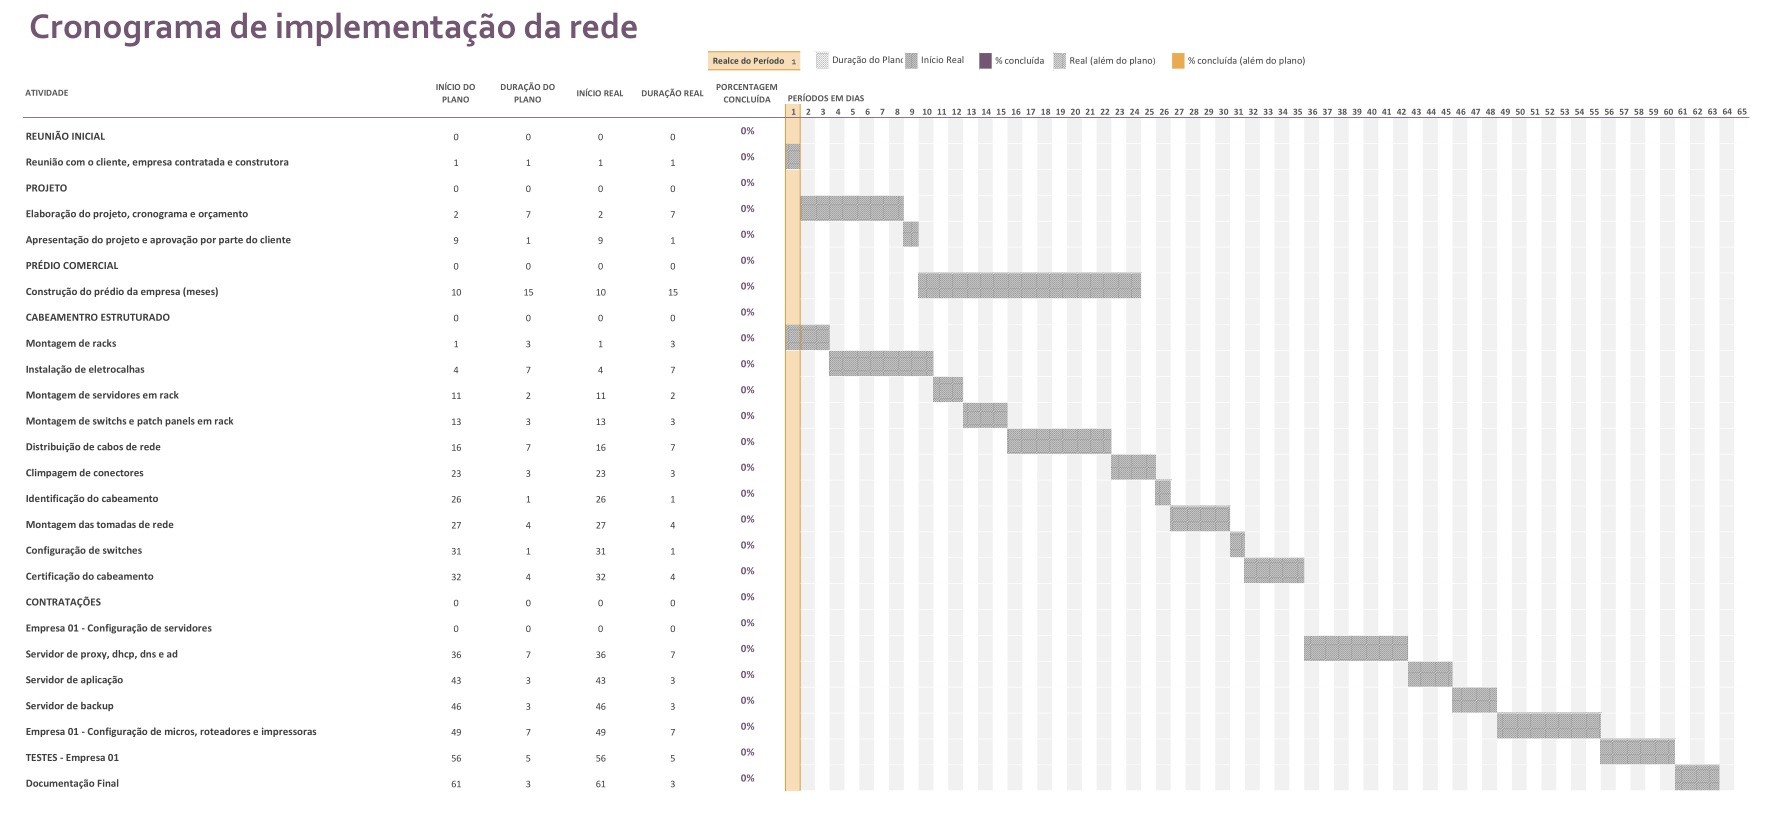
\includegraphics[height=\textwidth,angle=-90,scale=0.565]{crono}
	\caption{Cronograma para a execução do projeto.}
	\label{crono}
\end{figure}


\section{Plano de certificação}
Para a rede ser totalmente certificada, os canais e links serão testados eletricamente para atender a norma TIA-568-C.2. Os testes para o cabeamento metálico serão realizados com um aparelho certificador de rede.

Os testes serão:
\begin{itemize}
	\item Continuidade e sequência;
	\item Comprimento;
	\item Atenuação;
	\item NEXT - Paradiafonia - Near End CrossTalk;
	\item PSNEXT - Soma da paradiafonia - Power Sum NEXT;
	\item ELFEXT - Telediafonia - Equal Level Far - End CrossTalk;
	\item PSELFEXT - Somatória da telediafonia - Power Sum ELFEXT;
	\item Perda de retorno;
	\item Retardo do grupo ou tempo de atraso;
	\item Dispersão de atraso.	
\end{itemize}
A certificação será realizada após o término dos serviços prestados pela empresa contratada, dessa maneria a estrutura da rede estará completa, próximo do que seria em operação real. Para uso de parâmetro, a figura \ref{certificacao} abaixo indica os valores corretos para cada teste.

\begin{figure}[h!]
	\centering
	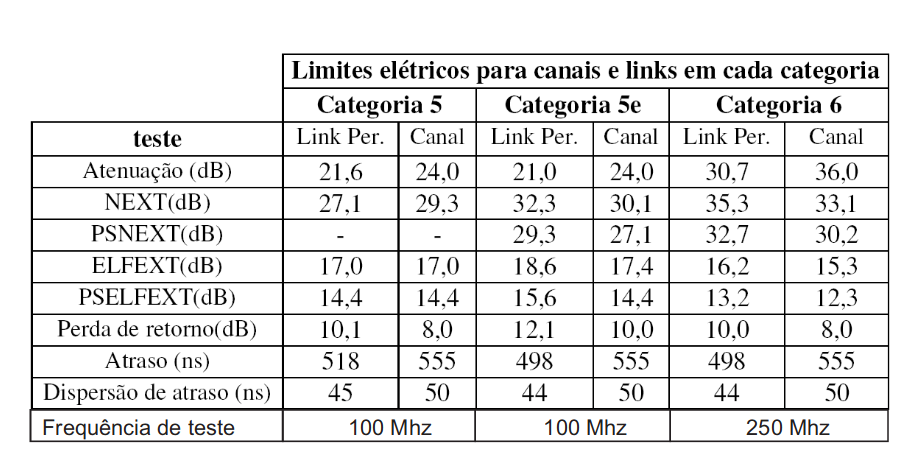
\includegraphics[scale=0.3]{certificacao}
	\caption{Valores em DB para referência nos testes.}
	\label{certificacao}
\end{figure}

O relatório da certificação será composto pelos testes de cada item apresentado, de maneira à apresentar a aprovação ou não do cabeamento estruturado e as correções necessárias para o correto funcionamento da rede.

\section{Plano de manutenção}

A empresa cliente optou por não contratar as revisões periódicas na estrutura, somente a necessidade de atendimento para eventuais problemas na rede e o contrato com a empresa contratante para o gerenciamento de servidores, computadores e impressoras.

\subsection{Plano de expansão}

A empresa apresentou nenhum plano para a expansão da estrutura de rede.

\section{Risco}
Os riscos do projeto que podem afetar a estrutura são:

\begin{itemize}
	\item Perda de dados: podem ocorrer por algum desligamento não programado dos servidores;
	\item Incêndio em data center: por alguma falha elétrica poderá acarretar em inicio de chamas na sala de TI;
	\item Colaboradores não autorizados: por acesso não definido de usuários podem comprometer a segurança dos dados.
\end{itemize}


\section{Orçamento}
Os orçamentos serão divididos em dois, um para os serviços necessários para o cabeamento estruturado da empresa e um de equipamentos para a rede. As tabelas \ref{tab9} e \ref{tab8} apresentam os valores do orçamento.


\begin{table}[h!]
	\centering
	\caption{Servicos prestados}
	\label{tab9} %com este label vc faz referencia no texto
\begin{tabular}{|c|c|c|c|}
\hline
\multicolumn{4}{|c|}{Servicos}                                                          \\ \hline
Mao de obra            & Duracao-Horas & Custo/H    & Total                             \\ \hline
Cabeamento Estruturado & 280           & R\$ 150,00 & R\$ 42000,00                      \\ \hline
Contratacao Empresa 01 & 200           & R\$ 90,00  & R\$ 18000,00                      \\ \hline
\multicolumn{3}{|l|}{TOTAL SERVICOS}                & \multicolumn{1}{l|}{R\$ 60000,00} \\ \hline
\end{tabular}
\end{table}










\newpage
\begin{table}[h!]
	\centering
	\caption{Orcamento-Equipamentos Passivos de Rede}
	\label{tab8} %com este label vc faz referencia no texto

\begin{tabular}{|c|c|c|c|c|c|}
\hline
\multicolumn{6}{|c|}{Equipamentos para a rede}                                                                                                                                                                                                                               \\ \hline
Equipamento                                                            & Marca             & Modelo                                                                                                                 & Qtd & Preco Un    & Total                              \\ \hline
Cabo UTP CAT6                                                          & Furukawa          & Caixa 305M                                                                                                             & 6   & R\$ 1597,00 & R\$ 9582,00                        \\ \hline
Patch Cords CAT6                                                       & Furukawa          & Cabo 1M                                                                                                                & 80  & R\$ 15,00   & R\$ 1200,00                        \\ \hline
Conector RJ-45                                                         & Furukawa          & \begin{tabular}[c]{@{}c@{}}Macho CAT6 Pacote \\ 50 Pecas\end{tabular}                                                  & 3   & R\$ 195,00  & R\$ 585,00                         \\ \hline
\begin{tabular}[c]{@{}c@{}}Modulo Tomada \\ para Rede\end{tabular}     & Fame              & \begin{tabular}[c]{@{}c@{}}RJ-45 CAT6 \\ 1 peca 8 vias\end{tabular}                                                    & 60  & R\$ 60,00   & R\$ 3600,00                        \\ \hline
Eletrocalhas                                                           & InfraEletrocalhas & \begin{tabular}[c]{@{}c@{}}150x100mm - \\ Perfuradas  3M\end{tabular}                                                  & 9   & R\$ 73,95   & R\$ 665,55                         \\ \hline
\begin{tabular}[c]{@{}c@{}}Eletrocalhas Curva \\ Vertical\end{tabular} & InfraEletrocalhas & \begin{tabular}[c]{@{}c@{}}Ext. 90- \\ 150x100mm\end{tabular}                                                         & 1   & R\$ 19,95   & R\$ 19,95                          \\ \hline
Suporte Omega                                                          & InfraEletrocalhas & 150x100mm                                                                                                              & 18  & R\$ 5,25    & R\$ 94,50                          \\ \hline
Patch Panels                                                           & Furukawa          & \begin{tabular}[c]{@{}c@{}}CAT6 24 posicoes \\ GIGALAN\end{tabular}                                                    & 4   & R\$ 762,51  & R\$ 3050,04                        \\ \hline
Rack Aberto 24U                                                        & Nacional Racks    & 19 - 1,27M x 0,67M                                                                                                     & 1   & R\$ 537,64  & R\$ 537,64                         \\ \hline
\begin{tabular}[c]{@{}c@{}}Rack Coluna \\ Padrao 24U\end{tabular}      & Nacional Racks    & 19 - 1,27M x 0,67M                                                                                                     & 1   & R\$ 361,89  & R\$ 361,89                         \\ \hline
Switch                                                                 & Dell              & Networking X1026                                                                                                       & 4   & R\$ 2199,00 & R\$ 8796,00                        \\ \hline
Servidor                                                               & Dell              & \begin{tabular}[c]{@{}c@{}}PowerEdge R230 |\\  1HD de 1TB | 8GB\end{tabular}                                           & 3   & R\$ 6199,00 & R\$ 18597,00                       \\ \hline
Computador                                                             & Dell              & \begin{tabular}[c]{@{}c@{}}Inspiron Small Desktop\\ -Intel Core i5 - 8GB - W10\\ Home + Monitor 21,5 pol.\end{tabular} & 4   & R\$ 4208,00 & R\$ 16832,00                       \\ \hline
Roteador                                                               & TP-Link           & AC1200 - Archer C50                                                                                                    & 2   & R\$ 218,71  & R\$ 437,42                         \\ \hline
Impressora                                                             & Brother           & \begin{tabular}[c]{@{}c@{}}Laser Duplex WiFi -\\  DCP-L2540DW\end{tabular}                                             & 1   & R\$ 1628,32 & R\$ 1628,32                        \\ \hline
\multicolumn{5}{|l|}{TOTAL EQUIPAMENTOS}                                                                                                                                                                                                & \multicolumn{1}{l|}{R\$ 65.987,31} \\ \hline
\end{tabular}
\end{table}
























Apresentados os valores, a tabela \ref{tab10} à seguir contém o orçamento total:

\begin{table}[h!]
	\centering
	\caption{Orcamento Total}
	\label{tab10} %com este label vc faz referencia no texto
\begin{tabular}{|c|c|}
\hline
Orcamento Total          & Valor         \\ \hline
Equipamentos para a rede & R\$ 65987,31  \\ \hline
Servicos                 & R\$ 60000,00  \\ \hline
TOTAL                    & R\$ 125987,31 \\ \hline
\end{tabular}
\end{table}










\newpage
\section{Recomendações}
Segue a lista abaixo com algumas recomendações para o correto funcionamento da estrutura de rede:

\begin{itemize}
	\item Manter a sala de TI refrigerada;
	\item Uso de câmeras para a segurança da sala de TI;
	\item Agendamentos periódicos para a manutenção da rede e equipamentos de informática.
\end{itemize}

\section{Referências bibliográficas}

\renewcommand\refname{} %%Referências bibliográficas}  
\bibliographystyle{ieeetr}
\bibliography{referencias}  

%% ***********************************************************************
 ================================================
%% ***********************************************************************

\end{document}